% !TeX root = ../sustechthesis-example.tex

\chapter[简介]{简介\label{section:introduction}}
\section[离子量子计算和量子测控]{量子计算和量子测控}
量子计算(Quantum Computing, QC)因其强大的计算能力和潜在的应用前景而受到广泛关注。
在量子算法的配合下,量子计算机在一些特定问题上相对于经典通用计算机有着显著优势,如大素数分解\cite[]{Shor_1997, Singleton_Jr_2023}、量子多体系统仿真\cite[]{Feynman_1982, Lloyd_1996}、加速搜索过程\cite[]{Grover_2002}等。
离子阱是当前最具发展前景的量子计算平台之一,它的实现需要多种学科领域的支持,其中测控系统处于十分核心的地位,它将系统涉及的其余各个部分联系起来,
% 给出特定的微波信号、激光信号等策略对量子比特进行调控并采集结果进行分析和处理
结合相应的控制策略以实现量子计算的各种操作。

% \subsection[量子计算]{量子计算}


和经典计算机的实现方式类似,量子计算机也采用\emph{比特(Bit)}作为计算单元来实现计算。与经典计算机使用的\emph{经典比特(Bit)}不同的是量子计算的计算单元是\emph{量子比特(Qubit)}。在量子计算机中,这个最小的计算单元通常被表示为:$\ket{0}$和$\ket{1}$。经典比特可能处于的状态只有两个,一般来说$0$(低电平)或$1$(高电平),而量子比特不仅可能处于$\ket{0}$态或$\ket{1}$态,还可能处于两者的概率叠加状态。采用\emph{狄拉克符号(Dirac-Notation)}的方式,一个量子比特可以被表示为概率叠加:$\ket{\phi}=a_0\ket{0}+a_1\ket{1}$,其中$|a_0|^2+|a_1|^2=1$。对于多个量子比特共同存在的情况,整个系统$(N-qubits)$的状态可以被表示为:
\begin{align}
    \ket{\phi}=a_0\ket{0\dots0}+\dots+a_{2^N-1}\ket{1\dots1}\nonumber
\end{align}

这就是所谓的\emph{量子叠加原理(Principle of Quantum Superposition, PQS)}\cite[]{Fedorov_Manko_2019}。这也是量子计算机的\emph{量子并行性(Quantum Parallelism)}这一强大特性的来源。
为了实现量子比特这个量子计算机的最小计算单元,我们必须有某种定义明确的二能级量子系统。David DiVincenzo对量子计算机的实现要素进行了总结\cite[]{DiVincenzo_2000}:
\begin{enumerate}
    \item 一个定义明确的二能级系统来编码量子比特;
    \item 足够长的相干时间来执行量子操作;
    \item 能够将量子比特近乎完美的初始化到确定性纯态;
    \item 定义的量子比特能够组合实现通用量子门;
    \item 接近完美的量子比特状态读出;
\end{enumerate}

以上的这些原则被用于选择合适的物理平台来进行量子计算的实现,经过筛选后目前已经被证明有实现通用量子计算机潜力的物理系统平台有:离子阱系统、超导系统、线性光学系统、硅基量子点、原子系统、拓扑系统等。

迄今为止,作为1995年提出的量子计算的第一个候选者的激光冷却\emph{离子阱系统(Ion trap system)}仍然是实现大规模量子计算机最有前途的平台之一。离子拥有相干时间极长\cite[]{Fisk_Sellars_Lawn_Coles_1997}的内部状态,它保证了出色的纠缠和初始化特性\cite[]{Blatt_Wineland_2008}。储存在单个离子中的的量子比特状态可以有长达几秒钟的寿命\cite[]{Langer_Ozeri_Jost_Chiaverini_DeMarco_Ben_Kish_Blakestad_Britton_Hume_Itano_et_al_2005},在\emph{动态解耦技术(Dynamic Decoupling Technology, DCT)}的帮助下这个寿命可以超过$10$分钟\cite[]{Wang_Um_Zhang_An_Lyu_Zhang_Duan_Yum_Kim_2017},这是在所有现有量子计算物理平台中保持最长的相干时间记录。关于纠缠态的制备,离子阱系统在2011年已经实现了$14$个纠缠态的制备\cite[]{Monz_Schindler_Barreiro_Chwalla_Nigg_Coish_Harlander_Hänsel_Hennrich_Blatt_2011},这个数字在2018年更新到了20\cite[]{Friis_Marty_Maier_Hempel_Holzäpfel_Jurcevic_Plenio_Huber_Roos_Blatt_et_al_2018}。同时,四量子比特多部纠缠态的存储时间达到$1.1$秒\cite[]{Kaufmann_Ruster_Schmiegelow_Luda_Kaushal_Schulz_von_Lindenfels_Schmidt_Kaler_Poschinger_2017}。
此外,运动自由度可以用于实现不同量子比特之间的通信,确保全量子比特连接\cite[]{Debnath_Linke_Figgatt_Landsman_Wright_Monroe_2016}。离子的状态也可以用几乎完美的效率读出\cite[]{Myerson_Szwer_Webster_Allcock_Curtis_Imreh_Sherman_Stacey_Steane_Lucas_2008},在此基础上可以构建高保真量子逻辑门\cite[]{Ballance_Harty_Linke_Sepiol_Lucas_2016}。
DiVincenzo的原始论文还为构建大规模量子计算机所需的量子通信指定了两个额外的标准:能平稳地进行量子比特和所谓的“飞行”量子比特之间的相互转换(例如光子,量子信息编码在偏振、频率或相位),以及将这些飞行量子比特从一个位置高保真地传输到另一个位置的能力。
% 如果目标是构建一个平稳的大规模量子计算机,这些标准并不重要,但对于包括量子网络在内的其它一些应用来说是十分必要的。面向构建一个平稳的大规模量子计算机所需的系统间长距离量子信息互换,
在这方面,离子阱领域中一些方案采用囚禁离子的中尺度模块之间的光子互连来实现量子处理器的互联\cite[]{Monroe_Raussendorf_Ruthven_Brown_Maunz_Duan_Kim_2014}。虽然离子本身不太可能作为长距离量子通信或量子网络的飞行量子比特,但离子和光子之间的高保真纠缠已被实现\cite[]{Moehring_Blinov_Madsen_Duan_Monroe_2004}。
总之,离子满足量子计算的五个主要DiVincenzo标准,也验证了将它们的量子信息转移到飞行量子比特的能力。事实上,早在2004,所有这些标准在离子量子比特平台基本上都得到满足\cite[]{Leibfried_DeMarco_Meyer_Lucas_Barrett_Britton_Itano_Jelenković_Langer_Rosenband_et_al_2003,Moehring_Blinov_Madsen_Duan_Monroe_2004}。

% \begin{figure}
%     \centering
%     \caption[离子阱量子计算的组成]{离子阱量子计算的四大组成部分\label{fig:quantum_computing_ion_trap_system}}
%     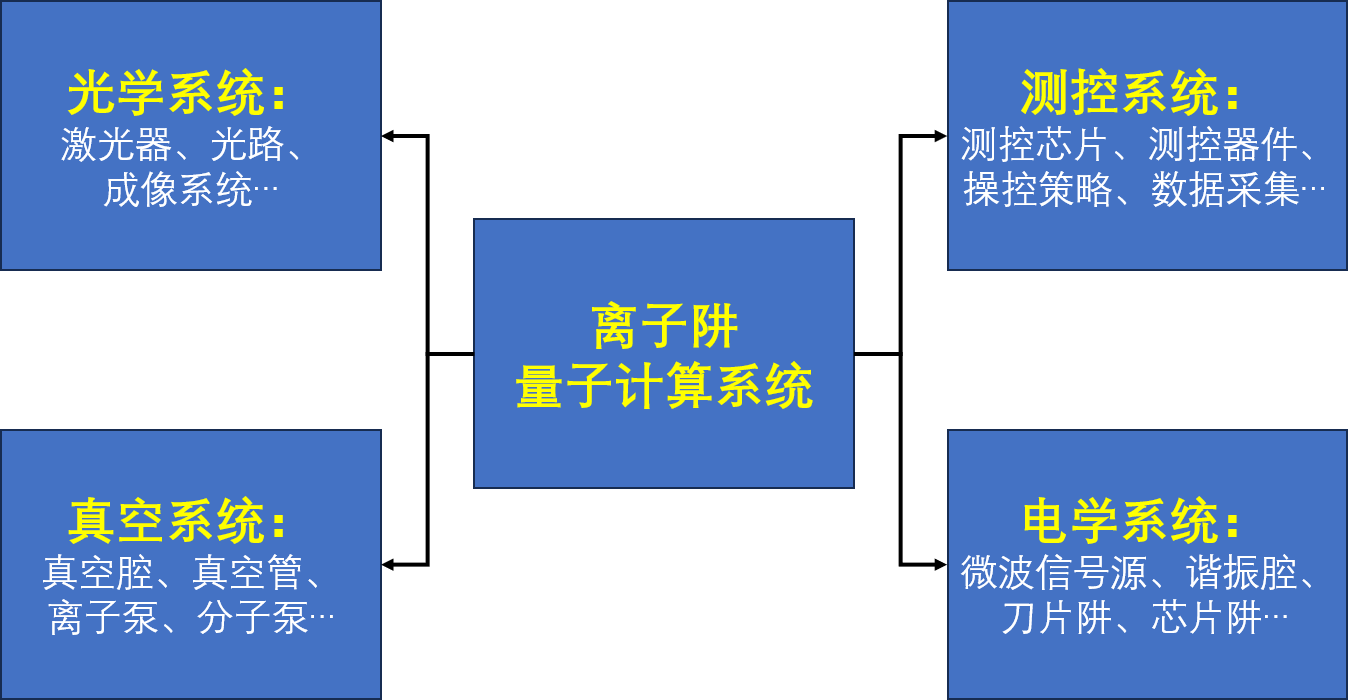
\includegraphics[width=0.8\linewidth]{quantum_computing_ion_trap_system}
% \end{figure}

离子阱量子计算系统是一个复杂综合的系统,
% 如图\ref{fig:quantum_computing_ion_trap_system}所示,
它主要由四大部分组成:1.  电学系统,主要包括微波信号源、谐振腔、阱电极等;2. 光学系统,主要包括激光器、由各类镜片组成的光路、成像系统等;3. 真空系统,主要包括真空腔、真空管、离子泵、分子泵等;4. 测控系统,主要包括测控芯片、测控器件以及配套的硬件和软固件等。想要实现基于离子阱的量子计算需要以上各大部分的相互配合。
其中量子测控系统处于十分核心的地位,它将电学、光学、真空等其余各个部分联系了起来,给出特定时序的微波、激光等信号对量子比特进行调控并采集结果进行分析和处理。
量子物理实验常常涉及到一些物理量的精确调控和测量,这既包括强度上的精确性,也包括时间上的精确性。随着量子技术的发展,量子物理实验系统也开始产生对数据处理、复杂流程控制和实时计算的需求。
% 不同于传统行业,量子物理实验系统对时间控制的精度和分辨率的要求在纳秒量级、延迟要求在百纳秒至数十微秒量级\cite[]{Ryan_Johnson_Ristè_Donovan_Ohki_2017,Guo_Qin_Schulz_2023},与当前微处理器的主频相当,这对量子物理实现的测控系统提出了很多新的要求。
具有更强实时性、更好可拓展性、集成度更高的量子测控系统对量子计算领域的发展至关重要。

% \subsection[量子测控]{量子测控}
现有的实时系统一般使用主频在数百MHz至GHz量级的通用微处理器或微控制器作为控制的主体,以计时器中断和时间片分配等方式实现实时控制。这一方案成立的前提是时间控制精度与指令执行频率之间有3-6个数量级的差异,可忽略处理器架构和中断系统的不确定性。
% 然而近来随着量子技术的发展,量子物理实验系统也开始产生对数据处理、复杂流程控制和实时控制的需求。
不同于传统行业,量子物理实验系统对时间控制的精度和分辨率的要求在纳秒量级、延迟要求在百纳秒至数十微秒量级\cite[]{Ryan_Johnson_Ristè_Donovan_Ohki_2017,Guo_Qin_Schulz_2023,junhua03},与当前微处理器的主频相当,从而前述的现有的实时控制方案难以满足需求。
因此早年在量子物理实验领域内,通常用FPGA(现场可编程门阵列)设计特定的时序脉冲发生器来产生高时间精度的脉冲序列,以此作为其它实验设备的触发信号,进行准确的时序控制。然而,这类方案的灵活性较差,只能产生预定的序列,无法在实验中对实验数据进行即时的处理,或根据实验的中间结果对后续的流程进行及时的调整\cite[]{junhua01}。随着量子算法发展,实验方案复杂,需在数十纳秒至数十微秒内处理中间结果并确定后续流程,简单的时序脉冲发生器已无法满足,实验测控系统需具备通用计算能力。

当前解决问题的思路是另置通用微处理器处理实验数据和产生时序。对于离子阱量子计算体系,量子物理高级实时基础设施(ARTIQ)\cite[]{Bourdeauducq_Jördens_Zotov_Britton_Slichter_Leibrandt_Allcock_Hankin_Kermarrec_Sionneau_et_al_2016}是控制量子物理实验的硬件、固件和软件的完整且免费开源框架。这也是目前大多数离子阱量子计算领域实验组所使用的测控系统技术方案。然而,ARTIQ的控制流架构使用在FPGA中实现的通用CPU,即所谓的软核CPU。这种方案虽然已经可以满足当前的离子阱量子实验需求,但是其进一步的拓展也受到多器件同步以及通信时延的影响而受限,并且对于对事件响应速率要求更高的超导量子比特实验难以保证可用性。针对超导量子计算的需求,来自UCSB/Google\cite[]{Chen_Sank_O’Malley_White_Barends_Chiaro_Kelly_Lucero_Mariantoni_Megrant_et_al_2012, Sank_Jeffrey_Mutus_White_Kelly_Barends_Chen_Chen_Chiaro_Dunsworth_et_al}、ETH Zurich\cite[]{Steffen_Salathe_Oppliger_Kurpiers_Baur_Lang_Eichler_Puebla_Hellmann_Fedorov_Wallraff_2013}、TU Delft\cite[]{Riste_Dukalski_Watson_Lange_Tiggelman_Blanter_Lehnert_Schouten_DiCarlo,Bultink_Rol_OBrien_Fu_Dikken_Dickel_Vermeulen_de_Sterke_Bruno_Schouten_et_al_2016}和Yale\cite[]{Ofek_Petrenko_Heeres_Reinhold_Leghtas_Vlastakis_Liu_Frunzio_Girvin_Jiang_et_al_2016}的研究者们也使用FPGA开发了自己的量子测控系统,且在进行将其应用到低温系统中的探索\cite[]{Homulle_Visser_Patra_Ferrari_Prati_Sebastiano_Charbon_2017, Conway_Lamb_Colless_Hornibrook_Pauka_Waddy_Frechtling_Reilly_2016},但是他们的这些软件都是不向整个量子计算社区开放的。
近几年来,随着量子计算领域的蓬勃发展,很多商业公司也逐步参与到量子测控系统的研发之中。Colm A. Ryan等人\cite[]{Ryan_Johnson_Ristè_Donovan_Ohki_2017}描述了雷声BBN技术公司为超导量子比特的动态量子信息处理实验开发的硬件、网关和软件。该方案的读出和控制平台都广泛地使用FPGA,使得量子比特控制系统的重构和迭代更加方便。但是该方案依赖两个独立器件(量子数字信号发生器(QDSP)和 任意波形发生器APS)的配合完成比特的读出和控制,其进一步的规模化拓展仍然受限于设备间的通信速率及设备的运算能力。
总体来说,这种面向量子领域的测控系统很难依靠经典CPU实现,当前大多数研究者开发的系统都是基于经典CPU+FPGA或者在FPGA上实现经典软核CPU的方式实现的,大都存在微处理器和时序脉冲发生器相互独立、同步困难的问题,会复杂化时序设计并产生时间浪费,影响其性能的进一步提升。
这些方案的另一问题在于,当系统规模较大,一个时序脉冲发生器无法控制整个系统时,就需要同时使用多个时序脉冲发生器,而一个微处理器同时处理过多的实验数据、同时控制过多的时序脉冲发生器,将不可避免的产生拥塞,这会进一步加剧前述的同步性问题。而如果同时使用多个微处理器,则不同微处理器之间的同步性又将成为问题。此外,当前主流的微处理器架构和指令集都是针对通用计算而优化的,主流的微处理器使用的通信协议都是针对高吞吐率而优化的,二者都难以实现精确的时序同步。
% 因此,一种能满足量子实时控制和信息处理的可大规模拓展的测控系统需求迫切,这种量子测控系统的实现可能需要专门设计强实时的微处理器架构以及相应的指令集,并且对于其大规模拓展也应具备强大的系统间同步能力。


尽管到目前为止离子阱量子计算发展迅速,但在实现通用量子计算机之前仍有许多问题有待解决。其中十分重要的一方面是量子测控系统\cite[]{Bourdeauducq_Jördens_Zotov_Britton_Slichter_Leibrandt_Allcock_Hankin_Kermarrec_Sionneau_et_al_2016,Chen_Sank_O’Malley_White_Barends_Chiaro_Kelly_Lucero_Mariantoni_Megrant_et_al_2012,Sank_Jeffrey_Mutus_White_Kelly_Barends_Chen_Chen_Chiaro_Dunsworth_et_al,Steffen_Salathe_Oppliger_Kurpiers_Baur_Lang_Eichler_Puebla_Hellmann_Fedorov_Wallraff_2013},一种能满足量子实时控制和信息处理的可大规模拓展的测控系统需求迫切,这种量子测控系统的实现可能需要专门设计强实时的微处理器架构以及相应的指令集,并且对于其大规模拓展也应具备强大的系统间同步能力。
除此之外,许多研究者也致力于芯片离子阱\cite[]{Mehta_Eltony_Bruzewicz_Chuang_Ram_Sage_Chiaverini_2014}、离子穿梭和规模化\cite[]{Monroe_Kim_2013, Sterling_Rattanasonti_Weidt_Lake_Srinivasan_Webster_Kraft_Hensinger_2014, Lee_Jeong_Park_Jung_Kim_Cho_2021}、光学集成\cite[]{Niffenegger_Stuart_Sorace_Agaskar_Kharas_Bramhavar_Bruzewicz_Loh_Maxson_McConnell_Reens_et_al_2020, Mehta_Zhang_Malinowski_Nguyen_Stadler_Home_2020}、多离子的单独寻址\cite[]{Ivory_Setzer_Karl_McGuinness_DeRose_Blain_Stick_Gehl_Parazzoli_2020}和量子比特纠错\cite[]{Cramer_Kalb_Rol_Hensen_Blok_Markham_Twitchen_Hanson_Taminiau_2016,Reichardt_2021}等技术,以实现最终目标——\emph{通用量子计算机(Universal Quantum Computer, UQC)}。

\section[论文章节结构介绍]{论文章节结构介绍}
% \textcolor{red}{简要阐述一下后续章节的主要内容...}
离子量子计算是当前最具发展前景的量子计算平台之一,它的实现需要电子学、光学、真空、测控等多种学科领域的支持。其中测控系统扮演着十分重要的角色,
% 测控系统涵盖着十分广阔的范围,包括测控核心板卡以及由其构成的如结合螺线管谐振腔的离子阱频率稳定、结合激光器的激光功率和激光拍频稳定等相关测控子系统。
以面向离子阱量子计算的实验测控系统研究为主旨,本文后续的章节结构如下:
\begin{itemize}
    \item 第\ref{section:quantum_computation}章,介绍囚禁离子量子比特的相关内容,以分析和明确量子物理实验对测控系统的切实需求。内容包括离子囚禁和量子化过程中涉及的在囚禁势场中的经典和量子运动,离子运动的量子化和离子与光场的耦合,离子(具体来说是镱离子)作为量子比特的编码和操控方案以及基于离子的通用量子门的构建;
    \item 第\ref{section:fpga_rtmq}章,引入了一种强实时性、可拓展性好、高度数字化和集成化的测控系统架构——RTMQ,以满足量子物理实验对测控系统的更高要求。同时也对RTMQ微处理器所配套设计的汇编指令集和多节点同步的实时通信链路系统进行了描述和分析,为后续量子测控板硬件设计及其功能拓展的实现和应用打下基础;
    \item 第\ref{section:helical}章,针对螺线管谐振腔这种离子囚禁系统中的重要射频器件进行了仿真、实验、建模、设计等方面的优化研究。谐振腔更高的Q值可以提高离子囚禁的稳定性和离子比特的保真度,针对螺线管谐振腔的Q值和频率运用有限元仿真软件HFSS进行了仿真模型的建立并与实验制作测量结果进行了验证。同时,针对旧有谐振腔惯用机械结构设计的缺点,给出了一种更加稳定易用、更模块化且装配方便的谐振腔机械结构设计;
    \item 第\ref{section:implementation}章,基于RTMQ测控系统架构(第\ref{section:fpga_rtmq}章),设计了一套适配的测控板硬件并实现了相应的功能外设。
    在此基础上,
    % 基于螺线管谐振腔(第\ref{section:helical}章)、激光器等器件并结合
    针对实验系统对量子比特操作保真度的实际需求,实现了RTMQ测控系统在离子量子计算应用场景下的几个关键子系统搭建和测试,包括离子阱频率稳定、激光功率稳定和激光拍频稳定等,展示了RTMQ系统的优越性。
    在此过程中也给出了高速通用数字PID和高速通用数字IIR滤波器的设计及FPGA实现。基于RTMQ架构的测控板的使用极大地促进了离子量子计算系统的数字化、集成化进程,同时也可以满足未来大规模通用量子计算对可拓展性的需求;
    \item 最后一章,对本论文进行了总结。
    % 并对离子量子计算及量子测控领域未来的发展进行了展望。
\end{itemize}